\documentclass[]{scrartcl}

\usepackage[utf8]{inputenc}
\usepackage{amssymb}
\usepackage{xcolor}
\usepackage{seqsplit} % splitting long seqs 
\usepackage{fontawesome} % cool icons
\usepackage{cmbright} % better fonts
\usepackage[most]{tcolorbox}
\usetikzlibrary{shapes.geometric}
\usepackage{scrlayer-scrpage}
\usepackage{xcolor}
\usepackage[section]{placeins}
\usepackage{listings}
\usepackage{longtable}
\usepackage{url}

\definecolor{plusgreen}{RGB}{17,87,64}
\newcommand{\ZZ}{\mathbb{Z}}


%%% exercise text formatting code - DO NOT CHANGE
\newcounter{exercise}
\newcounter{qid}[section]
\newcommand{\exerciseprefix}{prefix}
\newcommand{\questiontitle}{Questions}
\newcommand{\blockid}{B4}
\newcommand{\exname}{}
\newtcolorbox{exercisebox}[2][]{%
  colback=gray!5,
  colframe=plusgreen,
  fonttitle=\bfseries,
  title={\questiontitle},
  breakable,
  enhanced,
  sharp corners,
  boxrule=0.5pt,
  %before upper=\refstepcounter{exercise},
  overlay unbroken and last ={%
    % only draw points at end of box
    \if\relax\detokenize{#2}\relax\else
        \node[draw,ellipse,fill=orange,inner xsep=6pt, inner ysep=2pt,font=\small]
        at ([yshift=-2pt]frame.south) {#2 pts};
    \fi
  },
  #1
}



\lstdefinestyle{plusStyle}{
    basicstyle=\ttfamily\small,
    % --- Green Elements ---
    frame=single,
    rulecolor=\color{plusgreen},       % Frame border color
    numbers=left,
    numberstyle=\tiny\color{plusgreen}, % Line number color
    % ----------------------
    stepnumber=1,
    numbersep=8pt,
    breaklines=true,
    breakatwhitespace=false,
    postbreak=\mbox{\textcolor{plusgreen}{$\hookrightarrow$}\space}, % Green wrap arrow
    showstringspaces=false
}






\newcommand{\ctone}{CrypTool1}
\newcommand{\cttwo}{CrypTool2}
\newcommand{\ctonline}{CrypToolOnline}
\newcommand{\yoursolutionhere}{\textbf{YOUR-SOLUTION-HERE}}
\newcommand{\filename}[1]{\texttt{#1}}


\title{Homework Exercise Sheet 4\\Introduction to Cryptography \& IT-Security\\PS 511.088\\Summer Semester 2026}






%%%%%%%%%%%%%%%%%%%%%%%%%%%%%%%%%%%%%%%%%%%%%
% DO NOT MODIFY ANYTHING BEFORE THIS LINE IN THIS FILE %%%%%%%%%%%%
%%%%%%%%%%%%%%%%%%%%%%%%%%%%%%%%%%%%%%%%%%%%%%%%%%%%%%%%%%%%%%%%%
%%%%%%%%%%%% USE GROUP NAME FROM BLACKBOARD BELOW AND NO PERSONAL IDENTIFIABLE INFORMATION %%%%%%%%%%%%%%%%%%
\newcommand{\groupname}{YOUR-GROUP-NAME-FROM-BLACKBOARD-ONLY-HERE-NO-NAMES}
\author{\groupname}
%%%%%%%%%%%%%%%%%%%%%%%%%%%%%%%%%%%%%%%%%%%%%%%%%%%%%%%%%%%%%%%%%%%%%%%%%%


% format pagestyle below
\clearpairofpagestyles
%% Header
\chead{{\small \groupname}} %adjust font size as needed
%% Footer
\ifoot{{\small D. Simos, B. Garn, D. Schreiber}}
\cfoot{{\small University of Salzburg}}
\ofoot{{\small PS 511.088 SS2026}}
\pagestyle{scrheadings}


%%%%%%%%%%%%%%%%%
\begin{document}
\maketitle
\abstract{This is the forth homework exercise sheet for the proseminar \emph{Introduction to Cryptography and IT-Security} (PS 511.088) covering the block \emph{Classical Cryptography and Secure Protocols} to be completed before the proseminar on June 9, 2026 with a maximum of 20 points to be achieved. Submission deadline in Blackboard is June 2, 2026 at 12:59 PM. Late submissions will \textbf{not} be graded.

Use CrypTool software and/or SAGE to assist you in solving the exercises and the provided \LaTeX~code in the appendix to format your report, using the source \LaTeX~of the homework exercise sheet. Submit both resulting \texttt{tex/pdf} files in Blackboard. No other format is allowed.}
\date{}
\newpage


\pagebreak


\stepcounter{exercise}
\renewcommand{\exname}{DH}
\section*{PS-\blockid{}-E\theexercise: Diffie-Hellman (DH)}
The Diffie-Hellman key exchange (DHKE) is among the first published works on public key cryptography and has been integrated into many protocols. Its underlying mathematics are important to understand for their use in this cryptographic application of group theory. 


\stepcounter{qid}
\renewcommand{\exerciseprefix}{PS-\blockid{}-E\theexercise: \exname{}-Q\theqid}
\renewcommand{\questiontitle}{\exerciseprefix{}: Practical computing with DHKE}
\begin{exercisebox}{5}
You are intercepting a connection between Alice and Bob and received the public Diffie-Hellman prime and generator
\begin{itemize}
    \item $p = 37$
    \item $g = 6$
\end{itemize}
Next, you observe that Alice sends Bob the number $a = 36$ and Bob sends $b = 31$ to Alice.
\begin{enumerate}
    \item Find the key on which they agreed. 
    \item What makes the recovery of this key so easy? 
    \item From Alice's and Bob’s viewpoint, what would be a better choice of $g$?
\end{enumerate}
\end{exercisebox}

\paragraph{Answer:} \yoursolutionhere{}



\stepcounter{qid}
\renewcommand{\exerciseprefix}{PS-\blockid{}-E\theexercise: \exname{}-Q\theqid}
\renewcommand{\questiontitle}{\exerciseprefix{}: Practical computing with DHKE}
\begin{exercisebox}{1}
In the Diffie-Hellman key exchange, $g$ is chosen so that $2 \le g \le p - 2$. Give arguments why the values:
\begin{itemize}
    \item $g = p - 1$, 
    \item $g = p + 1$, 
\end{itemize}
are good or bad choices, respectively?
\end{exercisebox}

\paragraph{Answer:} \yoursolutionhere{}


\stepcounter{qid}
\renewcommand{\exerciseprefix}{PS-\blockid{}-E\theexercise: \exname{}-Q\theqid}
\renewcommand{\questiontitle}{\exerciseprefix{}: Practical computing with DHKE}
\begin{exercisebox}{2}
Digital signatures can be used to prevent a man-in-the-middle attack on Diffie-Hellman. Suppose that Alice and Bob already share a symmetric key $K$ before they begin the Diffie-Hellman procedure. Draw a diagram to illustrate a simple method Alice and Bob can use to prevent a man-in-the-middle attack.
\end{exercisebox}

\paragraph{Answer:} \yoursolutionhere{}



\pagebreak
\stepcounter{exercise}
\renewcommand{\exname}{DSS}
\section*{PS-\blockid{}-E\theexercise: Digital Signature Standard}
The Digital Signature Standard (DSS) was published by NIST and has been officially replaced. It represent \emph{early efforts} to advocate and push for widespread use of standardized cryptography. 

\stepcounter{qid}
\renewcommand{\exerciseprefix}{PS-\blockid{}-E\theexercise: \exname{}-Q\theqid}
\renewcommand{\questiontitle}{\exerciseprefix{}: Attack on optimized operational use of DSS}
\begin{exercisebox}{3}
Consider the DSS with the following parameters:
\begin{itemize}
    \item prime $q$;
    \item prime $p = aq + 1$ for some $a \in \ZZ$;
    \item element of order $q$ in $\ZZ_{p}^{*}$;
    \item a cryptographic hash function H;
    \item a secret key $x \in \ZZ_{q}$.
\end{itemize}
Consider the following mode of operations for applying DSS (in violation of the standard):
\begin{itemize}
    \item A User creates public/private key pair. 
    \item This user selects $k$ as required and further computes a pair $(k,r)$ such that $r \equiv \left( g^{k} \mod p \right) \mod q $
    \item This user \textbf{always} uses this pair (i.e., these two values $k$ and $r$) to compute any signatures.  
\end{itemize}
Assume that you have obtained - at least two - signatures that have been produced as described above. Show that in this case it is possible to perform an attack leading to universal forgery capabilities for the attacker by recovering the secret key $x$.
\end{exercisebox}

\paragraph{Answer:} {

For DSS, the signature is computed as

\[
s \equiv k^{-1}(H(m)+xr) \pmod q.
\]

Assume that two different messages $m_1$ and $m_2$ are signed using the same nonce $k$ and therefore the same value $r$.

Then the signatures satisfy

\[
s_1 \equiv k^{-1}(H(m_1)+xr) \pmod q
\]

and

\[
s_2 \equiv k^{-1}(H(m_2)+xr) \pmod q.
\]

Subtracting the two equations yields

\[
s_1-s_2
\equiv
k^{-1}(H(m_1)-H(m_2))
\pmod q.
\]

Thus,

\[
k
\equiv
(H(m_1)-H(m_2))
(s_1-s_2)^{-1}
\pmod q.
\]

After recovering $k$, we substitute it into the signature equation:

\[
s_1k
\equiv
H(m_1)+xr
\pmod q.
\]

Hence,

\[
xr
\equiv
s_1k-H(m_1)
\pmod q,
\]

and therefore

\[
x
\equiv
(s_1k-H(m_1))r^{-1}
\pmod q.
\]

Consequently, the attacker can recover the secret key $x$ from two signatures generated with the same nonce $k$.

Once $x$ is known, the attacker can generate valid signatures for arbitrary messages and therefore obtains \emph{universal forgery} capabilities.}

\stepcounter{qid}
\renewcommand{\exerciseprefix}{PS-\blockid{}-E\theexercise: \exname{}-Q\theqid}
\renewcommand{\questiontitle}{\exerciseprefix{}: Attack on optimized operational use of DSS}
\begin{exercisebox}{0.5}
In the context of the previous question, argue why the adversary has obtained universal forgery capabilities for signatures. List the concrete steps using an example. 
\end{exercisebox}

\paragraph{Answer:} {The attacker obtains \emph{universal forgery} capabilities because the attack described in Question~1 reveals the private signing key $x$.

The attack proceeds as follows:

\begin{enumerate}
\item Obtain two signatures
\[
(m_1,r,s_1)
\]
and
\[
(m_2,r,s_2).
\]

\item Since the same nonce $k$ was reused, the value $r$ is identical in both signatures.

\item Recover $k$ using
\[
k
\equiv
(H(m_1)-H(m_2))
(s_1-s_2)^{-1}
\pmod q.
\]

\item Recover the secret key
\[
x
\equiv
(s_1k-H(m_1))r^{-1}
\pmod q.
\]

\item Choose any new message $m_3$ and generate a valid DSS signature using the recovered private key $x$.
\end{enumerate}

Since signatures can now be generated for arbitrary messages, the attacker has achieved \emph{universal forgery}.}

\stepcounter{qid}
\renewcommand{\exerciseprefix}{PS-\blockid{}-E\theexercise: \exname{}-Q\theqid}
\renewcommand{\questiontitle}{\exerciseprefix{}: Attacking RSA signature}
\begin{exercisebox}{3}
You have intercepted the following message and RSA signature:
\begin{itemize}
    \item 150 dollars
    \item 56840167481593713576269217621738921774093
\end{itemize}
The signature was generated by using the str2num command of Sage to turn the message into an
integer $m$, using the following public key $(n,e)$:
\begin{itemize}
    \item $n = 2^{137} - 1$
    \item $e = 17$
\end{itemize}
Show how to use the \textbf{factor} command of sage to break this system and generate a forged signature for the following message:
\begin{itemize}
    \item 250 dollars
\end{itemize}
Demonstrate the forged signature using CrypTool 1: Menu Digital Signatures/PKI \faLongArrowRight Signature Demonstration (Signature Generation) $\ldots$
\end{exercisebox}

\paragraph{Answer:} 

Given the public key

\[
n = 2^{137}-1
\]

and

\[
e = 17,
\]

we first factor the modulus using Sage:

\begin{verbatim}
factor(n)
\end{verbatim}

which yields

\[
n =
5439042183600204290159
\cdot
32032215596496435569.
\]

Therefore,

\[
p = 5439042183600204290159
\]

and

\[
q = 32032215596496435569.
\]

Next, we compute Euler's totient:

\[
\varphi(n)=(p-1)(q-1).
\]

The private exponent is

\[
d=e^{-1}\pmod{\varphi(n)}.
\]

Using Sage:

\begin{verbatim}
phi = (p - 1)*(q - 1)
d = inverse_mod(e, phi)
\end{verbatim}

we obtain

\[
\varphi(n)=174224571863520493287776724605868623539744.
\]

\[
d =
40994016909063645479476876377851440832881.
\]

For the message

\begin{verbatim}
250 dollars
\end{verbatim}

we compute

\begin{verbatim}
m = str2num("250 dollars")
sig = power_mod(m, d, n)
\end{verbatim}

\[
m =
139566616181646573880489266.
\]

The forged RSA signature is

\[
\boxed{
125370169660687702452878304929998178247783
}.
\]

This signature can be successfully verified using the public key
\((n,e)\) in CrypTool 1.



\stepcounter{qid}
\renewcommand{\exerciseprefix}{PS-\blockid{}-E\theexercise: \exname{}-Q\theqid}
\renewcommand{\questiontitle}{\exerciseprefix{}: Theoretical aspects on RSA signature attack}
\begin{exercisebox}{0.5}
In the context of the previous question, argue why the adversary has obtained partial or universal forgery capabilities for signatures. List the concrete steps using an example. 
\end{exercisebox}
\paragraph{Answer:} {

In Question~3, the attacker factors the RSA modulus

\[
n = pq,
\]

which allows the computation of

\[
\varphi(n)
=
(p-1)(q-1)
\]

and subsequently the private exponent

\[
d
=
e^{-1}
\pmod{\varphi(n)}.
\]

Once the attacker knows $d$, signatures can be generated for arbitrary messages.

The RSA signing operation is

\[
\sigma
=
m^d
\pmod n.
\]

Verification is performed by checking

\[
\sigma^e
\equiv
m
\pmod n.
\]

For example, for the message

\begin{verbatim}
250 dollars
\end{verbatim}

the attacker computes

\[
m = \texttt{str2num("250 dollars")}
\]

and then

\[
\sigma = m^d \pmod n.
\]

The resulting signature is

\[
\sigma
=
125370169660687702452878304929998178247783.
\]

Since the attacker possesses the private signing key and can generate valid signatures for any chosen message, the attack results in

\[
\boxed{\text{Universal Forgery}}
\]

rather than merely

\[
\boxed{\text{Partial Forgery}}.
\]}

\pagebreak
\stepcounter{exercise}
\renewcommand{\exname}{TLS}
\section*{PS-\blockid{}-E\theexercise: Transport Layer Security}
The Transport Layer Security protocol is fundamental in modern network architectures and a major building block for modern Internet. Defining, implementing and deploying TLS is very complicated and there have been many security issues found in the past. The different versions of TLS have been specified in several RFCs that also point to other data such as the official TLS Cipher Suites list published by IANA (\url{https://www.iana.org/assignments/tls-parameters/tls-parameters.xhtml#tls-parameters-4}). 


\stepcounter{qid}
\renewcommand{\exerciseprefix}{PS-\blockid{}-E\theexercise: \exname{}-Q\theqid}
\renewcommand{\questiontitle}{\exerciseprefix{}: TLS Cipher Suites}
\begin{exercisebox}{0.5}
Consider the IANA list of official TLS Cipher Suites. 
\begin{itemize}
    \item Do all listed ciphers provide security?
    \item Do some ciphers provide 'more' security than others?
    \end{itemize}
\end{exercisebox}

\paragraph{Answer:} \yoursolutionhere{}


\stepcounter{qid}
\renewcommand{\exerciseprefix}{PS-\blockid{}-E\theexercise: \exname{}-Q\theqid}
\renewcommand{\questiontitle}{\exerciseprefix{}: TLS Cipher Suites}
\begin{exercisebox}{3}
A paranoid client wants to connect to a TLS server. For some reasons, the client prefers to avoid cryptographic standards from
the US Government and would like to rely on symmetric keys of at least 128 bits for his very secret transaction.
\begin{verbatim}
TLS_NULL_WITH_NULL_NULL
TLS_RSA_WITH_NULL_MD5
TLS_RSA_WITH_NULL_SHA
TLS_RSA_EXPORT_WITH_RC4_40_MD5
TLS_RSA_WITH_RC4_128_MD5
TLS_RSA_WITH_RC4_128_SHA
TLS_RSA_EXPORT_WITH_RC2_CBC_40_MD5
TLS_RSA_WITH_IDEA_CBC_SHA
TLS_RSA_EXPORT_WITH_DES40_CBC_SHA
TLS_RSA_WITH_DES_CBC_SHA
TLS_RSA_WITH_3DES_EDE_CBC_SHA
TLS_DH_DSS_EXPORT_WITH_DES40_CBC_SHA
TLS_DH_DSS_WITH_DES_CBC_SHA
TLS_DH_DSS_WITH_3DES_EDE_CBC_SHA
TLS_DH_RSA_EXPORT_WITH_DES40_CBC_SHA
TLS_DH_RSA_WITH_DES_CBC_SHA
TLS_DH_RSA_WITH_3DES_EDE_CBC_SHA
TLS_DHE_DSS_EXPORT_WITH_DES40_CBC_SHA
TLS_DHE_DSS_WITH_DES_CBC_SHA
TLS_DHE_DSS_WITH_3DES_EDE_CBC_SHA
TLS_DHE_RSA_EXPORT_WITH_DES40_CBC_SHA
TLS_DHE_RSA_WITH_DES_CBC_SHA
TLS_DHE_RSA_WITH_3DES_EDE_CBC_SHA
TLS_DH_anon_EXPORT_WITH_RC4_40_MD5
TLS_DH_anon_WITH_RC4_128_MD5
TLS_DH_anon_EXPORT_WITH_DES40_CBC_SHA
TLS_DH_anon_WITH_DES_CBC_SHA
TLS_DH_anon_WITH_3DES_EDE_CBC_SHA
TLS_RSA_WITH_AES_128_CBC_SHA
TLS_DH_DSS_WITH_AES_128_CBC_SHA
TLS_DH_RSA_WITH_AES_128_CBC_SHA
TLS_DHE_DSS_WITH_AES_128_CBC_SHA
TLS_DHE_RSA_WITH_AES_128_CBC_SHA
TLS_DH_anon_WITH_AES_128_CBC_SHA
TLS_RSA_WITH_AES_256_CBC_SHA
TLS_DH_DSS_WITH_AES_256_CBC_SHA
TLS_DH_RSA_WITH_AES_256_CBC_SHA
TLS_DHE_DSS_WITH_AES_256_CBC_SHA
TLS_DHE_RSA_WITH_AES_256_CBC_SHA
TLS_DH_anon_WITH_AES_256_CBC_SHA
\end{verbatim}
\begin{enumerate}
    \item Select the only two cipher suites from the list above which satisfy the security policy of the client. Notice that one of the two requires to authenticate a public key. Identify which one.
    \item Consider the cipher suite which requires public key authentication. Assume that an X.509 certificate is transmitted from the server to the client, but that the certificate authority is not known by the client. What happens? What is the typical reaction of the user?
    \item Compare the security of the two cipher suites. Are they considered secure today?
\end{enumerate}
\end{exercisebox}

\paragraph{Answer:} \yoursolutionhere{}


\stepcounter{qid}
\renewcommand{\exerciseprefix}{PS-\blockid{}-E\theexercise: \exname{}-Q\theqid}
\renewcommand{\questiontitle}{\exerciseprefix{}: openSSL message signing}
\begin{exercisebox}{1.5}
You have already seen how the signing process with RSA works using Cryptool 1 in a previous task. Now you are going to do this procedure using the openSSL utility in Cryptool Online. You can use the GUI or the shell commands directly.

\begin{enumerate}
    \item Go through the procedure of generating a key and and then sign the message "Hello world!" and the file signme.txt that is provided in the exercise materials and document your process.
    \item Compare the generated signatures. Are the signatures the same?
    \item Now use openssl to verify the signatures and document your process.
\end{enumerate}



\end{exercisebox}

\paragraph{Answer:} \yoursolutionhere{}





\newpage
\section*{Appendix: Instructions for Homework Sheet Preparation in \LaTeX}

\subsection{How to Include an Image}
A picture can be included in your document using the \LaTeX code used to obtain Figure \ref{fig:demo}.

\begin{figure}
    \centering
    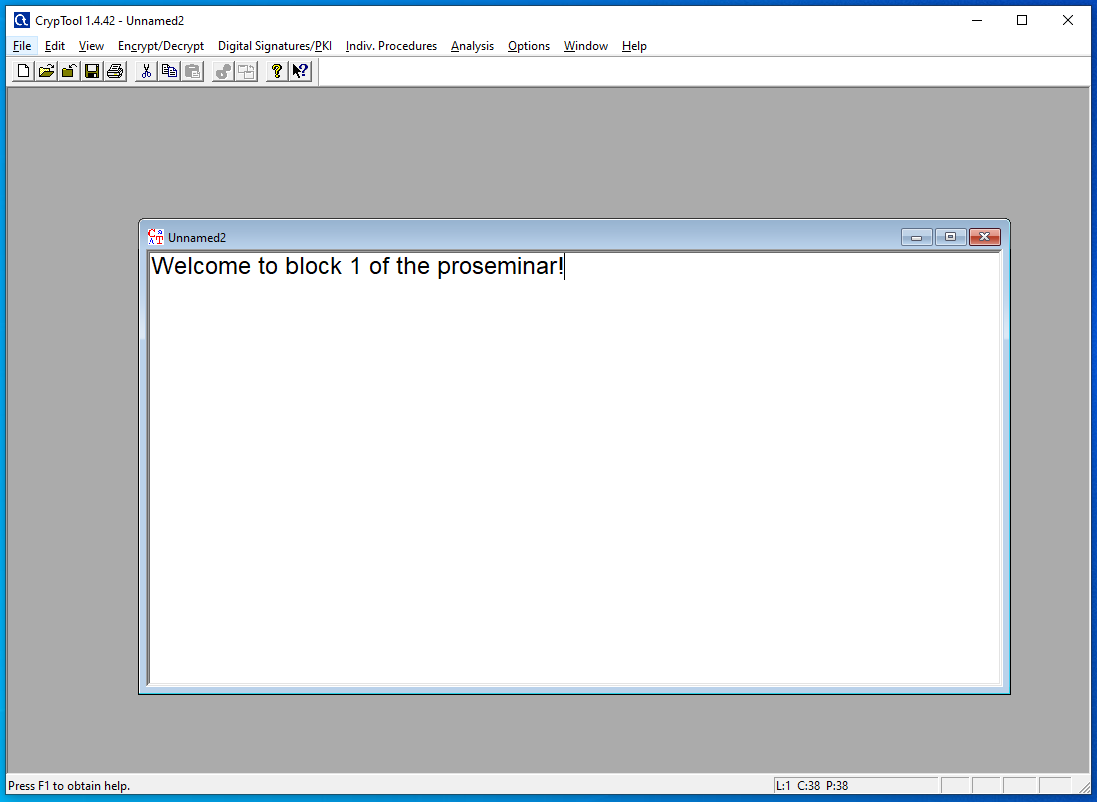
\includegraphics[scale=0.35]{figures/cryptool1.PNG}
    \caption{The code of this figure can be used when preparing your homework.}
    \label{fig:demo}
\end{figure}

\subsection{How to Include a Table}

A table can be included using the commands used to obtain Table \ref{tab:example}.

\begin{table}[ht]
    \centering
    \begin{tabular}{|c|c|c|}
    \hline
        Software & Assessment & Comments \\
        \hline
        Suite A & works well & internal use only \\
        \hline
        Suite B & freely usable & observe guidance document \\
        \hline
        Suite C & restricted & Requires compiler \\
        \hline 
    \end{tabular}
    \caption{Caption}
    \label{tab:example}
\end{table}

\subsection{How to List Data like Hexdumps}

Hexadecimal encoding provides a way to encode data in a machine and human-readable way. The code that has been used to generate Listing \ref{lst:example} can be used to include hex-data, including the one provided by \ctone{}. 
\begin{lstlisting}[style=plusStyle, caption={Example for how to include hex-data.},basicstyle=\tiny\ttfamily,label=lst:example]
50 63 D8 D0 D8 E4 FC F7 09 FB 1F 40 C1 99 E7 62 56 8A 20 77 B9 D6 F7 21 B3 61 F0 8D
96 AA 45 E3 A0 A5 11 97 58 17 2B 53 60 6D A3 2C A0 4C 2E 1F 5F 31 94 6A CC 09 28 8E
E0 0E 7C 23 2E 2F E3 E6 6A 02 AA D2 A7 41 80 6D AF 5D 72 63 0E AE A8 1F 3A 38 E3 91
74 56 B6 D7 59 C8 14 4B 0F C2 D8 9F 46 98 26 92 AF 5D 60 9E 5D AC 30 A1 DD 7A D1 95
49 AD 54 3C 93 B0 DF BC B2 57 83 AF F7 43 D8 98 0B 06 A4 6B 42 4C 8D 44 F4 7C BB B0
A6 B3 A2 7E 9C 11 D7 A6 98 23 EC 23 8E C8 AC FD 15 B0 2F 2B EC 49 25 B5 70 9C 0B D5
8A 24 5F 8C 7D 1A 32 E9 4C EF E7 B1 06 C7 D4 A2 C8 DA 01 15 99 E2 92 6B 0E DF 5B 36
15 2B 30 30 E0 5A A6 E0 80 2F 07 4F B4 4F 66 F8 17 A0 A3 72
\end{lstlisting}


\end{document}




